\section{Atividade 10}

\subsection{Identificação de Sistemas}

Nesta atividade, identificaremos o sistema representado pela função de transferência obtida na Atividade 3, utilizando a resposta ao degrau unitário. Aplicaremos os métodos de Harriot e Smith para a identificação de sistemas de segunda ordem e compararemos os resultados.

Para facilitar a análise, utilizamos um diagrama simples do sistema, onde escolhemos um degrau com amplitude 5, permitindo que a resposta mantivesse o valor normalizado em 1, evitando a necessidade de normalização posterior. Isso assegura que os resultados sejam diretamente interpretáveis.

A Figura \ref{fig:diagrama-sistema} apresenta a resposta ao degrau unitário do sistema massa-mola-amortecedor com os parâmetros \(M = 10\), \(C = 7\), e \(K = 5\). A resposta ao degrau é usada para identificar os parâmetros do sistema utilizando os métodos de Harriot e Smith.

\begin{figure}[h]
    \centering
    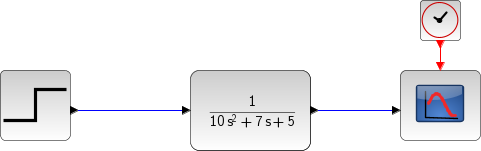
\includegraphics[width=0.8\textwidth]{atividades/10-atividade/assets/diagrama-sistema.png}
    \caption{Resposta ao degrau unitário do sistema massa-mola-amortecedor.}
    \label{fig:diagrama-sistema}
\end{figure}

A resposta ao degrau é marcada com pontos específicos utilizando a ferramenta DataTip, nos valores de 20\%, 60\%, 73\% e 100\%.

A Figura \ref{fig:sistema-identificado-forcado-normalizado} mostra a resposta ao degrau unitário do sistema massa-mola-amortecedor, com a identificação dos parâmetros baseada nos métodos de Harriot e Smith.

\begin{figure}[h]
    \centering
    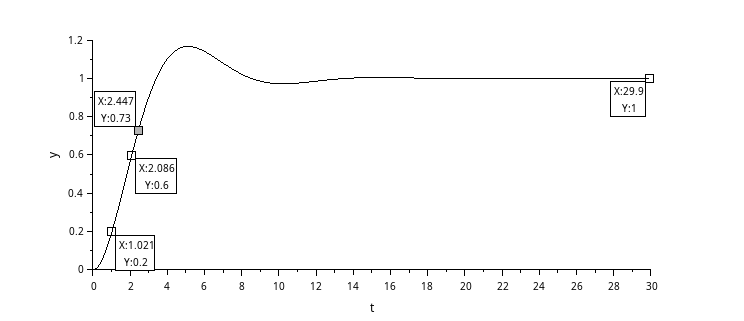
\includegraphics[width=0.8\textwidth]{atividades/10-atividade/assets/sistema-identificado-forcado-normalizado.png}
    \caption{Identificação dos parâmetros do sistema com a resposta ao degrau unitário.}
    \label{fig:sistema-identificado-forcado-normalizado}
\end{figure}


\subsection{Aplicação do Método de Harriot}

O Método de Harriot é utilizado para identificar os parâmetros de um sistema de primeira ordem a partir da resposta ao degrau. Neste método, a constante de tempo (\(\tau\)) e o ganho do sistema (\(K\)) são derivados da forma como o sistema responde a um degrau unitário. No entanto, nesta análise, o degrau aplicado teve amplitude 5, não unitária. Essa escolha foi feita para manter a resposta diretamente interpretável e evitar a necessidade de normalização posterior. Para aplicação do Método de Harriot, consideramos duas abordagens:

\begin{enumerate}
    \item \textbf{Utilização direta do degrau de amplitude 5:} Ao usar um degrau com amplitude 5, evitamos a normalização dos valores de saída. Isso simplifica a análise e mantém os dados experimentais mais próximos do sistema real.
    \item \textbf{Normalização para um degrau unitário:} Se tivéssemos aplicado um degrau unitário, seria necessário dividir todos os valores de saída pelo valor final esperado (\(5K\)). Este método ajusta a resposta para que a amplitude do degrau pareça unitária, permitindo a aplicação direta das fórmulas padrão do Método de Harriot.
\end{enumerate}

A constante de tempo crítica para a análise pelo Método de Harriot é calculada como:
\[
    t = 0.5 \cdot \frac{t_{73}}{1.3} = 0.5 \cdot \frac{2.449}{1.3} \approx 0.9419 \text{ segundos}
\]

Os pontos de resposta ao degrau utilizados para a análise são:
\begin{itemize}
    \item Para \(X = 1.022\), \(Y = 0.2\) (20\% do valor final).
    \item Para \(X = 2.094\), \(Y = 0.6\) (60\% do valor final).
    \item Para \(X = 2.449\), \(Y = 0.73\) (73\% do valor final).
    \item Para \(X = 29.9\), \(Y = 1\) (100\% do valor final).
\end{itemize}

\subsubsection{Limitação do Método de Harriot}

Uma limitação significativa do Método de Harriot é que ele é aplicável somente quando \(Y/KM > 0.26\) após a normalização para uma resposta ao degrau unitário. No caso em análise, o valor de \(Y/KM\) foi 0.175, que está abaixo do limite necessário. Além disso, o Método de Harriot é apropriado apenas para sistemas sobreamortecidos, enquanto o sistema em análise é subamortecido. Estas limitações sugerem que o Método de Harriot pode não fornecer uma identificação precisa dos parâmetros do sistema para esta resposta específica. Portanto, recomenda-se explorar métodos alternativos de identificação ou ajustar a configuração experimental para garantir que os requisitos do método sejam atendidos.

Com essa razão, podemos inferir características como o fator de amortecimento (\(\zeta\)) e a frequência natural (\(\omega_n\)) do sistema. Usando métodos padrão de identificação de sistemas, tal razão auxilia na determinação de parâmetros críticos que definem a dinâmica do sistema.

\begin{figure}[h]
    \centering
    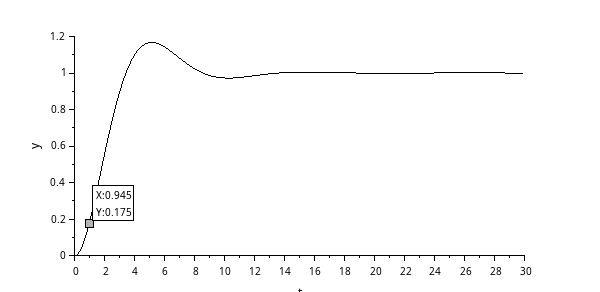
\includegraphics[width=0.8\textwidth]{atividades/10-atividade/assets/sistema-t73-identificado-nromalizacao-forcada.png}
    \caption{Identificação do sistema massa-mola-amortecedor utilizando o Método de Harriot.}
    \label{fig:sistema-t73-identificado-nromalizacao-forcada}
\end{figure}

Como observado na Figura \ref{fig:sistema-t73-identificado-nromalizacao-forcada}, a razão \(Y/KM\) foi de 0.175, indicando que o Método de Harriot não é aplicável neste caso. Este valor está abaixo do limite de 0.26, necessário para a aplicação eficaz do método.

\subsection{Aplicação do Método de Smith}

O Método de Smith utiliza a resposta ao degrau para identificar a frequência natural (\(\omega_n\)) e o fator de amortecimento (\(\zeta\)). A partir do gráfico da resposta ao degrau, podemos calcular esses parâmetros utilizando as equações correspondentes ao método.

Para calcular a razão entre os tempos, utilizamos a fórmula:
\[
    \frac{t_{20}}{t_{60}} = \frac{1.022}{2.086} \approx 0.461706
\]

Essa razão é então utilizada no gráfico do Método de Smith (Figura \ref{fig:analise-smith}), que relaciona \(\frac{t_{20}}{\tau}\) e \(\frac{t_{60}}{\tau}\) com \(\zeta\) e \(\tau\). Observa-se que a imagem tem dois eixos Y: um para \(\frac{t_{60}}{\tau}\) (à esquerda) e outro para \(\zeta\) (à direita). Este gráfico, no entanto, contém ruídos devido à sua obtenção via imagem e pode não ser totalmente preciso.

\begin{figure}[h]
    \centering
    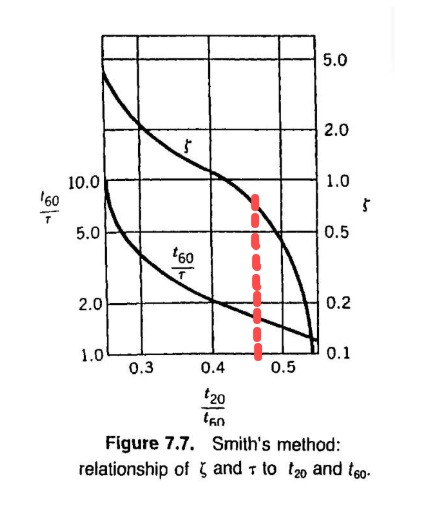
\includegraphics[width=0.8\textwidth]{atividades/10-atividade/assets/analise-smith.png}
    \caption{Gráfico utilizado no Método de Smith: relação entre \(\zeta\) e \(\tau\) com \(\frac{t_{20}}{\tau}\) e \(\frac{t_{60}}{\tau}\).}
    \label{fig:analise-smith}
\end{figure}

Para a análise, identificamos os seguintes pontos na resposta ao degrau:
\begin{itemize}
    \item Para \(X = 1.022\), \(Y = 0.2\) (20\% do valor final).
    \item Para \(X = 2.094\), \(Y = 0.6\) (60\% do valor final).
    \item Para \(X = 2.449\), \(Y = 0.73\) (73\% do valor final).
    \item Para \(X = 29.9\), \(Y = 1\) (100\% do valor final).
\end{itemize}

Com a razão \(\frac{t_{20}}{t_{60}} \approx 0.461706\), localizamos no gráfico o valor correspondente de \(\frac{t_{60}}{\tau}\), que é aproximadamente 1.8. Utilizando este valor e o tempo \(t_{60}\) conhecido, podemos encontrar \(\tau\) pela fórmula:
\[
    \tau = \frac{t_{60}}{1.8}
\]

Substituindo o valor de \(t_{60}\):
\[
    \tau \approx \frac{2.086}{1.8} \approx 1.159
\]

Finalmente, com \(\tau\) e utilizando a relação gráfica, podemos inferir o fator de amortecimento \(\zeta\) e a frequência natural \(\omega_n\) do sistema. No entanto, devido à natureza da análise gráfica via imagem, há uma incerteza associada aos valores obtidos.

Instanciando os valores encontrados na função de transferência do sistema, temos:
\[
    G(s) = \frac{Kp}{\tau^2 s^2 + 2 \zeta \tau s + 1}
\]

Onde, com os valores obtidos:
\[
    G(s) = \frac{Kp}{(1.159)^2 s^2 + 2 \zeta (1.159) s + 1}
\]


\subsubsection{Limitações do Método de Smith}

A análise com o Método de Smith realizada a partir da imagem do gráfico introduz incertezas devido aos possíveis ruídos e imprecisões na leitura dos valores. Para uma identificação mais precisa, recomenda-se utilizar gráficos gerados diretamente a partir dos dados experimentais sem a necessidade de interpretação visual de uma imagem.



\subsection{Comparação dos Métodos e Conclusão}

Ao comparar os métodos de Harriot e Smith, observa-se que cada método possui suas limitações específicas. O Método de Harriot é aplicável principalmente a sistemas sobreamortecidos e apresentou limitações significativas quando aplicado a um sistema subamortecido, como o analisado. Além disso, a razão \(Y/KM\) calculada foi insuficiente para a aplicação eficaz do método.

Por outro lado, o Método de Smith, apesar de ser mais adequado para sistemas subamortecidos, introduziu incertezas devido à análise gráfica baseada em uma imagem, resultando em possíveis ruídos e imprecisões.

Dado o caso de uso existente e as formas como os métodos foram aplicados, não é possível fazer a identificação dos parâmetros do sistema de uma forma confiável e aceitável. Portanto, é melhor concluir que não foi possível realizar uma identificação precisa e confiável do sistema do que fazer afirmações com muitas dúvidas. Recomenda-se a utilização de métodos alternativos ou ajustes na abordagem experimental para alcançar uma identificação mais precisa e segura.
